\documentclass{article}
\usepackage{tikz}

\begin{document}


\begin{figure}[!h]
%\begin{center}
\scalebox{0.9}{

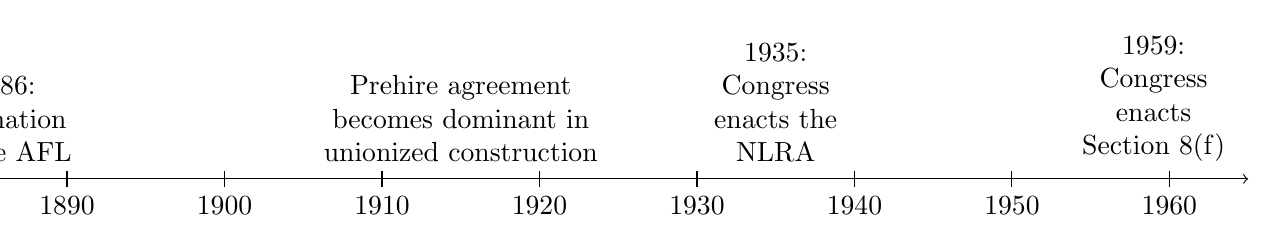
\begin{tikzpicture}[trim left=2.5cm]%, trim right=2cm]
  % Draw horizontal line
  \draw[<->] (0,0) -- (18,0);
  % Draw vertical lines and nodes
  \foreach \x/\year in {1/1880,3/1890,5/1900,7/1910,9/1920,11/1930,13/1940,15/1950,17/1960} {
    \draw (\x,-0.1) -- (\x,0.1);
    \node[below] at (\x,-0.1) {\year};
  }
  % Events
  \draw (2.2,0.1) node[above,text width=2cm,align=center] {1886: Formation of the AFL};% -- (2.2,-0.2);
  \draw (8,0.1) node[above,text width=4cm,align=center] {Prehire agreement becomes dominant in unionized construction};% -- (8,-0.2);
  \draw (12,0.1) node[above,text width=2cm,align=center] {1935: Congress enacts the NLRA};% -- (12,-0.2);
  \draw (16.8,0.1) node[above,text width=2cm,align=center] {1959: Congress enacts Section 8(f)};% -- (16.8,-0.2);
\end{tikzpicture}
}
%\end{center}

%\begin{tikzpicture}
%  % Draw horizontal line
%  \draw[->] (0,0) -- (10,0);
%  % Draw vertical lines and nodes
%  \foreach \x/\year in {0/2000,2/2005,4/2010,6/2015,8/2020,10/2025} {
%    \draw (\x,-0.1) -- (\x,0.1);
%    \node[below] at (\x,-0.1) {\year};
%  }
%  % Draw events
%  \draw (1,0) node[above] {Event 1} -- (1,-0.2);
%  \draw (3,0) node[above] {Event 2} -- (3,-0.2);
%  \draw (5,0) node[above] {Event 3} -- (5,-0.2);
%  \draw (7,0) node[above] {Event 4} -- (7,-0.2);
%  \draw (9,0) node[above] {Event 5} -- (9,-0.2);
%\end{tikzpicture}


\end{figure}
\end{document}
